\documentclass{swfcthesis}
\usepackage{xcolor}
\usepackage{hyperref}
\usepackage[utf8]{inputenc}
\usepackage{listings}
\usepackage{verbatim}
\usepackage{tikz}
\usetikzlibrary{shapes.geometric, arrows}
\usetikzlibrary{positioning}


\tikzstyle{startstop} = [rectangle, rounded corners, minimum width=3cm, minimum
height=1cm,text centered, draw=black, fill=red!30]

\tikzstyle{io} = [trapezium, trapezium left angle=70, trapezium right angle=110, minimum
width=5cm, minimum height=1cm, text width = 4cm, draw=black, fill=blue!30]

\tikzstyle{process} = [rectangle, minimum width=3cm, minimum height=1cm, text centered,
text width = 3cm, draw=black, fill=orange!30]
\tikzstyle{decision} = [diamond, minimum width=3cm, minimum height=1cm, text centered, draw=black, fill=green!30]

\tikzstyle{arrow} = [thick,->,>=stealth]


\addbibresource{thesis.bib}    % 参照教程自己去写一个.bib文件

\begin{document}
\cite{os_wiki}
\cite{china_2025}
\cite{30_os}

\Title{RongOS --- 一个简单操作系统的实现}
\Author{蒲启元}
\Advisor{王晓林}
\AdvisorTitle{讲师}
\AdvisorInfo{王晓林,男,49岁,硕士,讲师,毕业于英国格林尼治大学,分布式系统专业,现任西
  南林业大学计信学院教师,执教Linux、操作系统、网络技术等方面的课程,有丰富的Linux教学和系
  统管理经验。}
\Month{六}
\Year{二〇一八}
\Univ{西南林业大学}
\School{计算机与信息科学学院}      %院系名称
\Subject{计算机科学与技术专业}    %专业名称(比如 电子信息工程专业)
\Docname{本科毕业(设计)论文}    %本科?研究生?
\Abstract{操作系统管理着计算机的硬件和软件资源,它是向上层应用软件提供服务(接口)的核心系
  统软件,这些服务包括进程管理,内存管理,文件系统,网络通信,安全机制等。操作系统的设计与
  实现则是软件工业的基础与内核。为此,在国务院提出的《中国制造2025》中专门强调了操作系统的
  开发。但长期以来,操作系统核心开发技术都掌握在外国人手中,技术受制,对于我们的软件工业来
  说很不利。本文拟从零开始设计开发一个简单的操作系统,包括boot loader,中断,内存管理,图
  形接口,多任务,以及在这个系统上的几个小应用等。尽管这个系统很简单,但它为自主开发操作系
  统做了一个小小的尝试。}
\Keywords{操作系统,开发,自主}
\Acknowledgments{首先我想感谢我的老师,王晓林。大学期间,他给了我很多指导,包括专业方面和
  上大学的意义等。很多时候,他对学生的要求看起来都是不近情理的,但正是通过这个“痛苦”的过程,
  我锻炼了坚强的意志,和战胜困难的信心。谢谢你,王老师。我最想感谢的是我的女友,她容忍我在
  完成这个设计时的很多个夜晚不陪她,给我支持,鼓励我,不抱怨。所以我愿意把这个简单操作系统
  命名为RongOS, 蓉便是她名字的最后一个字。谢谢你,我最亲爱的。}
\enTitle{The implement of a simple OS --- RongOS}
\enAuthor{Qiyuan Pu}
\enUniv{Southwest Forestry University}
\enSchool{School of Computer and Information Science} %英文院系名称
\enAbstract{Operating system manages the sources of hardware and software, it lie in the
  core of the system software and provide service(interface) to upper application. These
  service including process management, memory management, file system, network
  communication, security mechanism etc. The design and implement of operating system is
  the foundation and core of software industry. Therefore, <<Made in China 2025>>
  emphasize the development of operating system that put forward by The State Council. For
a long time, however, the kernel development technology grasped in the hand of foreigner,
it's bad for our software industry cause of limited technology. So this article will
design and develop a simple operating system, including boot loader, interrupt, memory
management, graphic interface, multitasking, and some little application depend on this
system. In spite of the simple of this system, it's a small trying for autonomous
development operating system.}
\enKeywords{operating system, development, autonomous}

%%% 下面六行不要动!
\makepreliminarypages% 封面
\frontmatter          
\tableofcontents     % 目录
\listoffigures       % 插图目录
\listoftables        % 表格目录
\mainmatter
\chapter{Introduction}

\section{Background}
\label{sec:background}


\section{Preliminary Works}

\subsection{Development Environment}
\label{sec:devel-envir}

Operating System: Debian 4.11.0-1-amd64 \\
\hspace*{0.8cm}Debug System: QEMU emulator version 2.8.1(Debian 1:2.8+dfsg-7)\\
\hspace*{0.8cm}Emacs version: GNU Emacs 25.2.2

\subsection{Tools}
\label{sec:tools}

Some tools used to develop RongOS, see
tools.\footnote{\url{https://github.com/Puqiyuan/RongOS/tree/master/Tools}}.

\subsection{Install}
\label{sec:install}

Debian System: there is a small
tutorial.\footnote{\url{http://cs2.swfc.edu.cn/~wx672/lecture_notes/linux/install.html}}\\
\hspace*{0.8cm}QEMU, for my x86\_64 architecture: 
\begin{lstlisting}[language=bash]
     $ sudo apt-get install qemu-system-x86_64
\end{lstlisting}

Note that the tools is exe formate, so on Debian system, you need to install wine:
\begin{lstlisting}
     $ sudo apt-get update
     $ sudo apt-get install wine
\end{lstlisting}

Maybe you also need to add i386 architecture cause of AMD64 on your machine to use \hspace*{0.8cm}these tools:
\begin{lstlisting}
     $ sudo dpkg --add-architecture i386
     $ sudo apt-get update
\end{lstlisting}


\begin{comment}
\subsection{表格示例}

下面是一个表格的例子:

\begin{table}[!ht]
  \centering
  \begin{tabular}{|r|c|l|}
    \hline
    Hello&world&Hello, world!\\
    \hline
    Hello&world&Hello, world!\\
    \hline
  \end{tabular}
  \caption{表格示例}
  \label{tab:hello}
\end{table}
\end{comment}


\chapter{Design}

\section{Top Level Design}
\label{sec:top-level-design}

\section{Detailed Design}
\label{sec:detailed-design}

\subsection{Boot Loader}
\label{sec:boot-loader}


The below is the flowchart of boot loader program:

  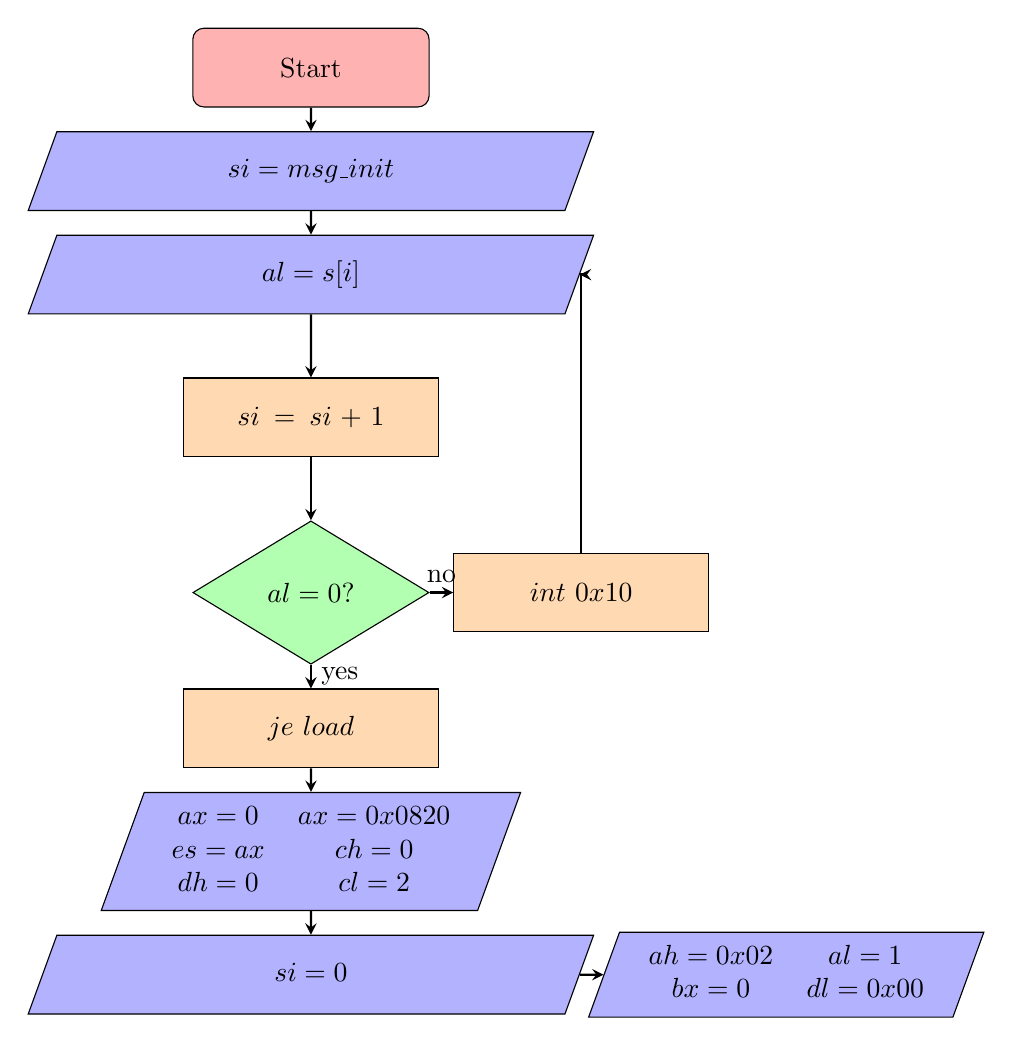
\begin{tikzpicture}[node distance=0.3cm]
    \node (start) [startstop] {Start};
    \node (in1) [io, below=of start, align=center]
    {
      \begin{tabular}{c}
        $si=msg\_init$
      \end{tabular}
    };
    \node (in2) [io, below=of in1,align=center]
    {
      \begin{tabular}{c}
        $al=s[i]$
      \end{tabular}
    };
    \node (pro1) [process, below=of in2, yshift = -0.5cm] {$si=si+1$};
    \node (dec1) [decision, below=of pro1, yshift= -0.5cm] {$al=0?$};
    \node (pro2) [process, right=of dec1] {$int\ 0x10$};
    \node (pro3) [process, below=of dec1] {$je\ load$};
    \node (in3) [io, below=of pro3, align=center]
    {
      \begin{tabular}{cc}
        $ax=0$ & $ax=0x0820$ \\
        $es=ax$ & $ch=0$ \\
        $dh=0$ & $cl=2$ \\
      \end{tabular}
    };
    \node (in4) [io, below=of in3, align=center]
    {
      \begin{tabular}{c}
        $si=0$
      \end{tabular}
    };
    \node (in5) [io, right=of in4, align=center]
    {
      \begin{tabular}{cc}
        $ah=0x02$  & $al=1$\\
        $bx=0$ & $dl=0x00$
      \end{tabular}
    };
%    \node (pro4) [process, below=of in5] {$int\ 0x13$};
    
 %   \draw[arrow] (in5) -- (pro4);
    \draw[arrow] (in4) -- (in5);
    \draw[arrow] (in3) -- (in4);
    \draw[arrow] (start) -- (in1);
    \draw[arrow] (in1) -- (in2);
    \draw[arrow] (in2) -- (pro1);
    \draw[arrow] (pro1) -- (dec1);
    \draw[arrow] (dec1) -- node[anchor=south] {no}(pro2);
    \draw[arrow] (pro2) |- (in2);
    \draw[arrow] (dec1) -- node[anchor=west] {yes} (pro3);
    \draw[arrow] (pro3) -- (in3);
  \end{tikzpicture}



\chapter{Implementation}

\section{Boot Loader}

\subsection{Chose Disk}
\label{sec:chose-disk}

There are many ways to boot a operating system, from hard disk, USB, floppy disk etc. I
chose floppy disk, although it is out of date. For my purpose is that develop a simple
operating system, pay my attention on how to development. The structure of floppy disk is
simple and for my simple operating system it's enough.

\subsection{The Structure of Floppy Disk}
\label{sec:struct-floppy-disk}

This picture show the inside of floppy disk:
\begin{figure}[!ht]
  \centering
  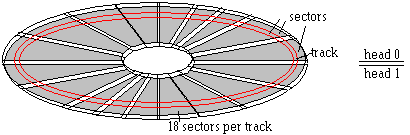
\includegraphics[width=.5\textwidth]{flpy1}
  \caption{Floppy Disk Structure}
  \label{fig:flpy1.png}
\end{figure}

The floppy store information in two sides. There are $80$ cylinders from the outermost to
the core in each side, numbering $0$, $1$, ..., $79$. The head can assign be $0$ or $1$,
representing two sides of floppy. When specify head number and cylinder number, forming a
ring, named track in jargon. The track is large so we divide it to 18 small parts, named
sector. A sector can store $512$ byte. So the capacity of a floppy is:

$$18 * 80 * 2 * 512 = 1474560 Byte = 1440 KB.$$

The IPL(Initial Program Loader) in C0-H0-S1(cylinder 0, head 0, sector 2), and the next
sector is C0-H0-S2.


\subsection{Flowchart of Boot Loader}
\label{sec:flowch-boot-load}





\subsection{Codes and Comments of Boot Loader}
\label{sec:codes-comments}


\inputminted[linenos=true]{nasm}{./ipl10.nas}

\section{32-bit Mode and Import C Codes}


\section{Screen Display and Text}

\section{Control Mouse}


\section{Memory Management}

\section{Making Window }

\section{Timer}

\section{Multitasking}

\section{Command Line Window}

\section{API}

\section{OS Protection}

\section{Graphics Processing}

\section{Window Operation}

\section{Application Protection}

\section{File Operation}

\section{Some Applications}

\section{Prospects and Shortages}

%%% 正文部分到此结束。下面是『参考文献』、『指导教师简介』、『鸣谢』、『附录』

%% 不要动下面四行!
\Appendix{}
\printbibliography[heading={bibintoc},title={参考文献}] % 输出参考文献
\advisorinfopage{}                 % 输出指导教师简介
\acknowledgmentspage{}             % 输出鸣谢

%%% 下面是附录部分,可以没有。

%\chapter{我也不知道为什么要写附录} %附录一

%可以参考模版目录中的 appendix.tex 文件来写。

%\chapter{主要程序代码} %附录二

% 插入程序代码

% 也可以这样
\end{document} % 结束。不要动下面几行!

%%% Local Variables:
%%% mode: latex
%%% TeX-master: t
%%% End:
